%%%%%%%%%%%%%%%%%%%%%%%%%%%%%%%%%%%%%%%%%%%%%%%%%%%%%%%%%%
\section{Previous Work}
\label{sec:previousWork}
%%%%%%%%%%%%%%%%%%%%%%%%%%%%%%%%%%%%%%%%%%%%%%%%%%%%%%%%%%
%\begin{figure}
%   {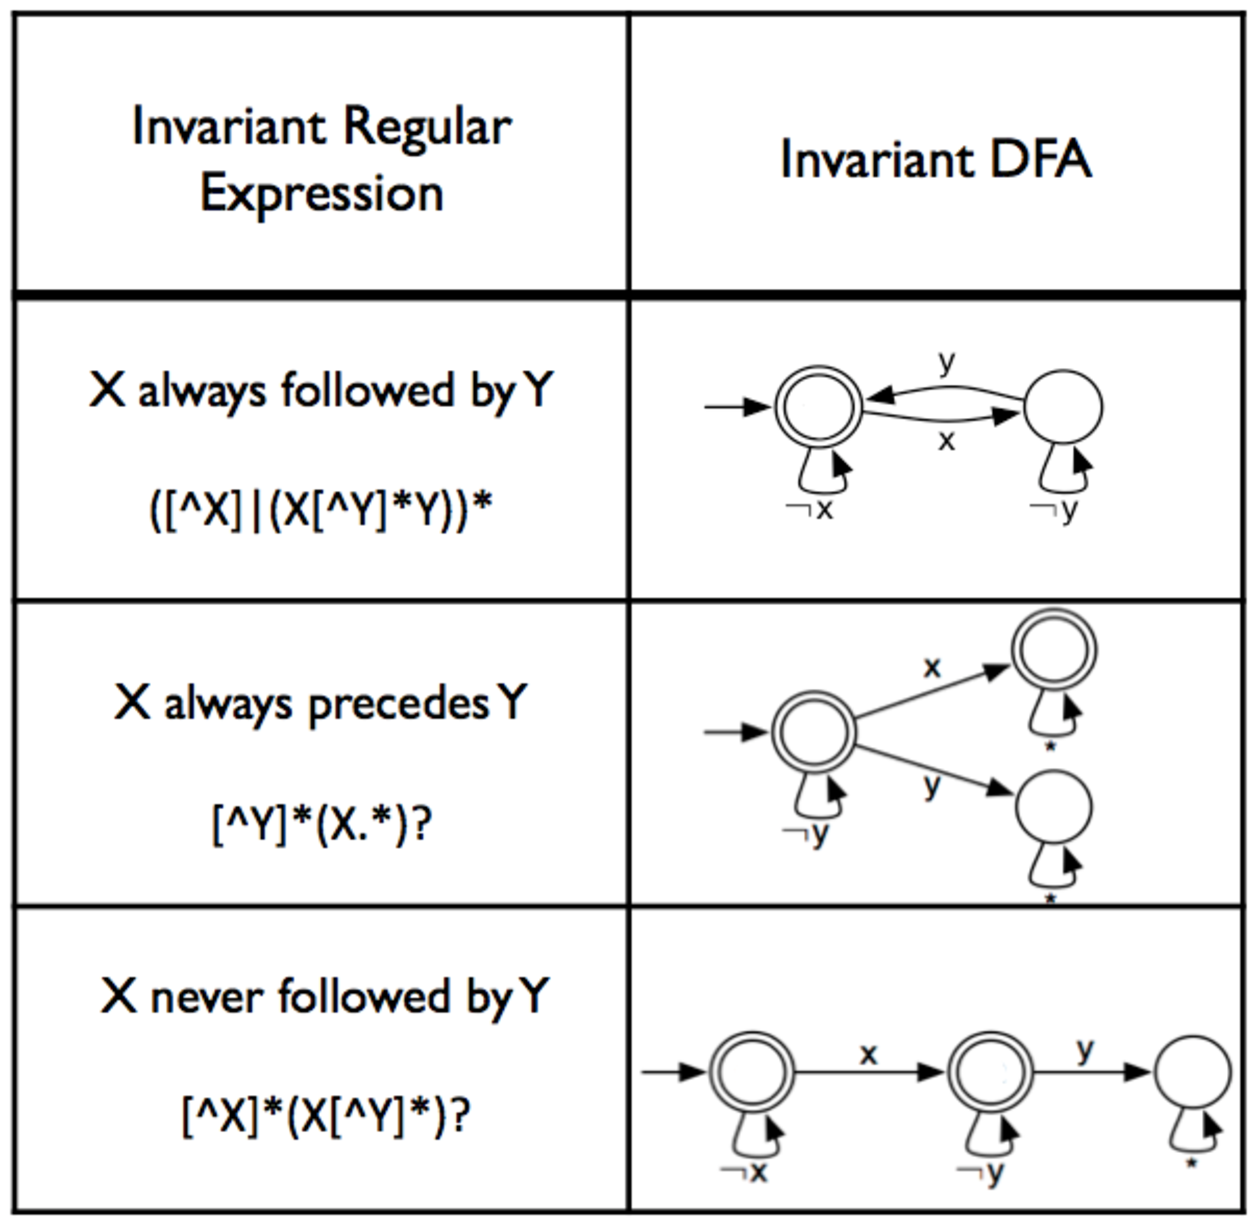
\includegraphics[width=\columnwidth]{fig/invRegexDfa.pdf}}
%   \caption{The regular expressions used to translate each invariant type into
%   an
%   invariant DFA.
%    } 
%   \label{fig:invRegDfa}
%\end{figure}
Previous work on this task has almost entirely been rule-based~\cite{HeidelTime}~\cite{SUTime}. The current state of the art approaches use a combination of regular-expression matching and hand-written interpretation functions to ground temporal expressions. These hand-built approaches are very domain-specific; they have a difficult time when applied to domains other than the one they were built for. Moreover, the complexities of natural language are often lost on these systems. Nested or hierarchical expressions are easy to handle when taking a parsing approach designed to deal with these phenomena, but these types of phrases can cause more rigid rule-based systems to fail. For example, phrases such as \emph{the third Wednesday of each month} or \emph{the second month of last year} are easier to ground using a parsing approach. 

While most of the work in this area has been on deterministic systems, one notable exception is ParsingTime~\cite{ParsingTime}. This system learned to parse from temporal phrases to logical forms, but is limited in that it doesn't take context into account. Their system uses a PCFG to parse the phrases to a logical form, then executes the form to get a result. However, their approach only looks at the temporal phrase itsef; it doesn't have any signal from the context in which the phrase appeared, such as verb tense or the result of parsing previously uttered phrases.

Previous work has shown that using CCG for semantic parsing can be successful. Zettlemoyer and Collins~\cite{LukeFirstPaper} used CCG to map from text queries to logical forms, achieving state-of-the-art results on a number of datasets. In much of the previous work using CCG, the parse itself is used as a query to a database, which can be evaluated directly. In this work, however, the parse is latent; we execute the parse using a deterministic algorithm, as our signal comes from the fully ground date or duration. Other approaches have used a learning approach for building the lexicon used to parse. In this work, we are using a hand-built lexicon, for greater coverage and to enable future work in building a joint model of detection and parsing.

%%%%%%%%%%%%%%%%%%%%%%%%%%%%%%%%%%%%%%%%%%%%%%%%%%%%%%%%%%%
\subsection{TempEval}
%%%%%%%%%%%%%%%%%%%%%%%%%%%%%%%%%%%%%%%%%%%%%%%%%%%%%%%%%%%
Within SemEval, TempEval-2 and, more recently, TempEval-3 were competitions held that included a task on grounding temporal expressions. The dataset they released includes gold extents, types and values for the temporal phrases in a set of documents. Within this dataset there are four types, \begin{inparaenum}[\itshape 1\upshape)] \item \texttt{date} (such as \texttt{1987-07-05} or \texttt{2013-Q3}), \item \texttt{time} (simply a date with a time, such as \texttt{1987-07-05T9}, for \emph{9 am July 5th, 1987}), \item \texttt{set} (such as \texttt{XXXX-QX}, for \emph{every quarter}), and \item \texttt{duration} (such as \texttt{P100Y}, for \emph{one hundred years}).\end{inparaenum} The values are more varied, as they represent more of the information the phrase grounds to. For example, the phrase \emph{July 5th, 1987} grounds to the value \texttt{1987-07-05}.

This paper and the results section deal with the dataset from the task A of the TempEval competitions. 
